El filtro Colorizar resalta los colores de la imagen de acuerdo al color predominante en un bloque de 3x3 píxeles según la siguiente regla:

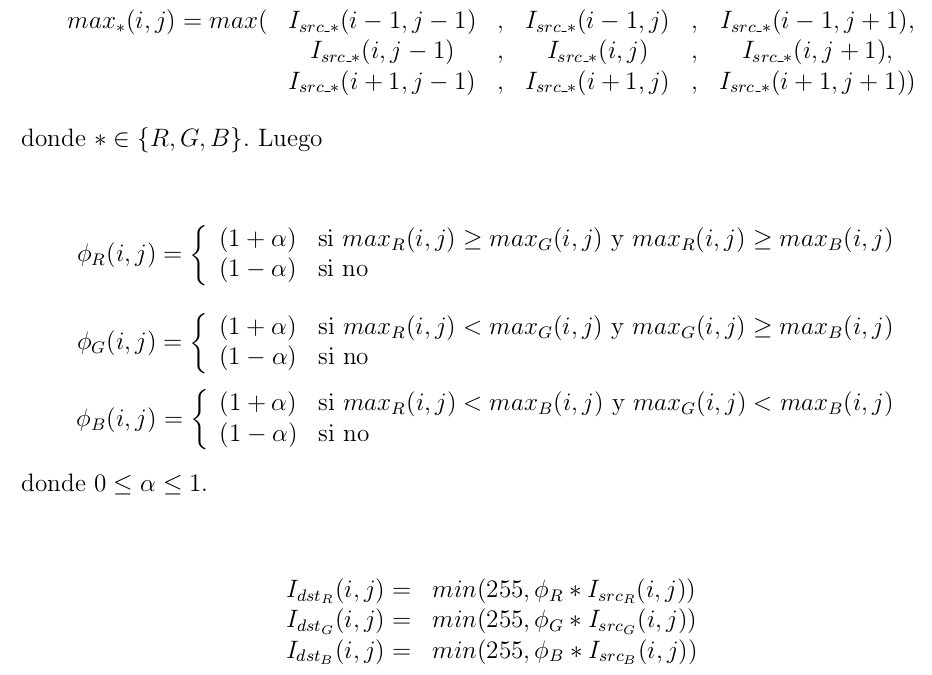
\includegraphics[width=\textwidth]{colorizar.jpg} 

\subsubsection{Implementación en C}

Se recorre la imagen con dos ciclos anidados de pixel en pixel (3 bytes) ignorando la primer y última fila y columna, calculando el valor de cada color del pixel destino.
Para calcular ese valor hay una función para el menor, mayor y $\phi$, lo que hace que además de traer los 8 píxeles que lo rodean, se hagan 15 llamados a funciones con su correspondiente costo de acceso a memoria.

\subsubsection{Implementación en Assembler}

En este filtro, como cada pixel ocupa 3 bytes y requiere tener datos de su predecesor y siguiente, se traen de a 5 píxeles y se ignora un byte.
Como en los demás filtros se hacen 2 ciclos anidados pero con ciertos detalles:
\begin{itemize}
\item En la altura empieza en 0 y va hasta height - 2, ya que en cada iteración se traen 3 filas.
\item En el ancho se trae primero desde el 0 y se ignora el último byte, pero en las siguientes iteraciones se ignora el primer byte, esto es para evitar pasarse y traer bytes que no pertenezcan a la imagen.
\item Al escribir en el destino, se escriben solamente 9 bytes nuevos (3 bytes), estos se colocan en la parte más significativa para no pasarse al escribir los bytes. Por esto se deben guardar los últimos 7 bytes de la iteración anterior para completar el registro y no pisar datos ya procesados.
\end{itemize}

En cada iteración se traen 16 bytes en 3 registros para tener suficiente como para procesar 3 píxeles.
El método para procesar 1 pixel consiste en calcular los máximos, luego comparar, calcular $\phi$ y, por último, multiplicar por $\pm$ $\alpha$ según corresponda:

\begin{pseudocodigo}
	\STATE maximos(regSrc, regDst) \{
	\INDSTATE[2] $regSrc = \{Basura, p1b, p1g, p1r, p2b, p2g, p2r, p3b, p3g, p3r, Basura, Basura, Basura, Basura, Basura, Basura\}$
	\INDSTATE[2] xmm3 = unpackLower(regSrc)
	\INDSTATE[2] xmm4 = unpackLower(xmm3)
	\INDSTATE[2] xmm5 = unpackLower(shiftRight(xmm3, 6))
	\INDSTATE[2] xmm4 = max(xmm4, xmm5)
	\INDSTATE[2] xmm3 = unpackLower(unpackLower(shiftRight(regSrc, 6)))
	\INDSTATE[2] regDst = max(xmm4, xmm3) \COMMENT{regDst = $\{Basura, MaxB, MaxG, MaxR\}$}
    \STATE \}
\end{pseudocodigo}

\begin{pseudocodigo}
	\STATE maximos(regLinea0, xmm6)
	\STATE maximos(regLinea1, xmm7)
	\STATE xmm6 = max(xmm6, xmm7)
	\STATE maximos(regLinea2, xmm7)
	\STATE xmm6 = (float) max(xmm6, xmm7) \COMMENT{xmm4 = $\{Basura, MaxB9, MaxG9, MaxR9\}$}
	\STATE pixelActual = (float) unpackHigher(unpackLower(regLinea1)) \COMMENT{Valores del pixel actual}
	
	\COMMENT{Hago shuffle para que me queden alineados y comparo}
	\STATE xmm6 = $\{Basura, MaxR, MaxG, MaxR\}$
	\STATE xmm7 = $\{Basura, MaxB, MaxB, MaxG\}$
	\STATE xmm8 = xmm6 $\geq$ xmm7
	\STATE $\phi$R = maxR $\geq$ maxG $\land$ maxR $\geq$ maxB
	\STATE $\phi$G = maxR $\textless$ maxG $\land$ maxG $\geq$ maxB
	\STATE $\phi$B = maxR $\textless$ maxB $\land$ maxG $\textless$ maxB
	\STATE reg$\phi$ = $\{Basura, \phi$B, $\phi$G, $\phi$R $\}$
	\STATE signo = reg$\phi$ $\land$ 0x80000000800000008000000080000000
	\STATE reg$\alpha$ = $\{ Basura, \alpha, \alpha, \alpha\}$
	\STATE signed$\alpha$ = reg$\alpha$ $\land$ $\neg$ signo \COMMENT{Queda $\alpha$ negativo en donde no se cumpla $\phi$}
	\STATE dst = pixelActual + pixelActual * signed$\alpha$ \COMMENT{Equivalente a pixelActual * (1 $\pm$ $\alpha$)}
	
\end{pseudocodigo}

Esto se repite para los otros 2 píxeles que puedo procesar por iteración y se acomodan, primero los 7 valores más significativos de la iteración anterior y luego los 9 bytes nuevos para escribir en la imagen destino.

\subsubsection{Resultados}

En la implementación en C, debido a los píxeles vecinos y las llamadas a funciones, se realizan, al menos, 25 accesos a memoria por cada pixel en la imagen destino.
En cambio en la implementación en ASM, para un bloque de 3 píxeles se realizan 4 accesos a memoria, 3 lecturas y una escritura. Por lo tanto debería ser al menos 18 veces más rápido.

Ejecutamos ambos filtros 100 veces cada uno y estos son los resultados obtenidos:

\begin{center}
    \begin{tabular}{|l|l|l|}
        \hline
         & Implementación C & Implementación en asm  \\
        \hline
        Duración promedio (en ciclos de clock) & 556 480 896        & 13 323 085 \\
        \hline
    \end{tabular}
\end{center}

Como se puede observar, la implentación en asm es $\sim$42 veces más rápida, lo que corrobora la hipótesis. La mejora mucho más significativa podemos verla analizando el código ASM generado por el gcc:
Variables locales auxiliares generan muchos más accesos a memoria por función, cosa que en el código ASM evitamos completamente sabiendo que pueden realizarse únicamente con registros.